\documentclass[a4paper, 10pt, final, garamond]{book}
\usepackage{cours-preambule}

\titleformat{\item}{}{\arabic{item})}{.5em}{}{}
\titleformat{\subitem}{}{\arabic{item}) \alph{subitem} --}{.5em}
{}{}

\makeatletter
\renewcommand{\@chapapp}{Devoir surveill\'e -- num\'ero}
\makeatother

\begin{document}
\setcounter{chapter}{6}

\chapter{Commentaires sur le DS n\degree7}

\begin{NCprop}[width=\linewidth]{\centering\bfseries\ Rappel des malus}
    Chacune des lettres suivantes sur vos copies sont des malus de \num{1}
    point.\smallbreak
    \begin{minipage}{0.50\linewidth}
        \begin{itemize}
            \item A~: application numérique mal faite~;
            \item V~: confusion ou oubli de vecteurs~;
            \item M~: marge inexistante ou trop petite~;
            \item Q~: question mal ou pas indiquée~;
        \end{itemize}
    \end{minipage}
    \begin{minipage}{0.50\linewidth}
        \begin{itemize}
            \item U~: unité manquante ou mauvaise~;
            \item H~: homogénéité non respectée~;
            \item S~: chiffres significatifs non respectés~;
            \item $\f$~: loi physique fondamentale brisée.
        \end{itemize}
    \end{minipage}
\end{NCprop}

\section{Commentaires généraux}

DS à 40, assez moyen. Note moyenne à 10/20. Total malus~: \textbf{170}, c'est
énormissime. Jusqu'à \textbf{11} points de malus sur une copie (et plusieurs
vers 8, 9) et même des exercices à points négatifs… On compte 1 seule personne
sans un seul malus, pour un total de \textbf{0} points de bonus. Plus grand gain
de place par rapport au DS06~: 24. Plus grande perte de place~: -15 places.

Prochain DS, malus G pour gâchis de papier (copies vides). Soyez raisonnables.

\begin{center}
    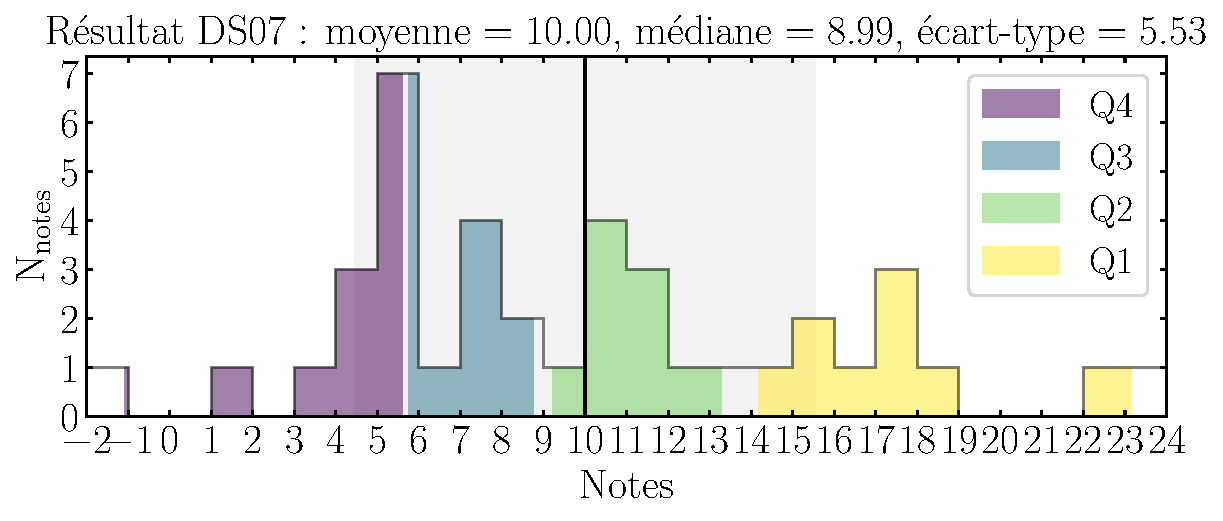
\includegraphics[width=.8\linewidth]{res_DS07.pdf}
\end{center}
\vspace*{-20pt}

\section{Exercice 1 \hfill \textcolor{red}{/18}}
\begin{enumerate}
  \item Établissez bien vos systèmes~!! Il y a deux flotteurs, donc chacun est
    immergé de moitié ce que vous trouvez en n'en supposant qu'un.
    \hfill \textcolor{ForestGreen}{/10}
  \item \textbf{Utilisez le bras de levier~!!}
    \hfill \textcolor{ForestGreen}{/5}
  \item Une puissance est en Watts.
    \hfill \textcolor{ForestGreen}{/3}
\end{enumerate}

\section{Exercice 2 \hfill \textcolor{red}{/41}}
\begin{enumerate}
  \item Le Newton n'est pas une unité SI…
    \hfill \textcolor{ForestGreen}{/10}
  \item \textbf{Utilisez le bras de levier, bis~!!}
    \hfill \textcolor{ForestGreen}{/15}
  \item RAS.
    \hfill \textcolor{ForestGreen}{/3}
  \item Rares sont les copies ayant bien traité cette question. Votre intuition
    physique est à utiliser judicieusement~: le vent pousse \textbf{forcément}
    vers la droite…
    \hfill \textcolor{ForestGreen}{/8}
  \item RAS sur toute la suite~; connaissez vos définitions.
\end{enumerate}

\section{Exercice 3 \hfill \textcolor{red}{/42}}
\begin{enumerate}
  \item ~
  \begin{framed}
      \begin{center}
          \huge
          La force de \textsc{Lorentz} est $q\Ef$~!!
      \end{center}
  \end{framed}
    Pas de $mq\Ef$ ou que sais-je…
    \hfill \textcolor{ForestGreen}{/4}
  \item Ça se démontre que le mouvement est plan…
    \hfill \textcolor{ForestGreen}{/6}
  \item RAS.
    \hfill \textcolor{ForestGreen}{/3}
  \item RAS.
    \hfill \textcolor{ForestGreen}{/3}
  \item Il faut savoir utiliser le gradient ou la définition de l'énergie
    potentielle à partir du travail élémentaire.
    \hfill \textcolor{ForestGreen}{/8}
  \item Il faut \textbf{expliquer votre tracé}~!
    \hfill \textcolor{ForestGreen}{/17}
\end{enumerate}

\section{Exercice 4 \hfill \textcolor{red}{/32}}
\begin{enumerate}
  \item Ne vous trompez pas de sens.
    \hfill \textcolor{ForestGreen}{/4}
  \item Ne faites pas n'importe quoi avec les applications numériques~:
    \textbf{littéral avant numérique}~! Je ne corrige pas les expressions qui ne
    sont pas littéralement lisibles (en plus d'un malus A). Attention aux
    chiffres significatifs.
    \hfill \textcolor{ForestGreen}{/7}
  \item Vous n'êtes pas attentif-ves à l'énoncé~: on \textit{a} de l'acide
    lactique dans le corps, c'est forcément un \textbf{réactif}. Pour savoir
    quelle réaction se produit, faire un diagramme en p$K_a$.
    \hfill \textcolor{ForestGreen}{/8}
  \item Ne confondez pas quantité de matière et concentration. $\xi$ avancement
    molaire, $x$ avancement volumique. Un tableau d'avancement se rédige aussi
    de manière littérale. Les A.N. ne se font qu'à la fin des questions.
    \hfill \textcolor{ForestGreen}{/11}
  \item RAS.
    \hfill \textcolor{ForestGreen}{/2}
\end{enumerate}

\section{Problème \hfill \textcolor{red}{/84}}
\begin{enumerate}
    \item Soyez attentif-ves~: on ne commence \textbf{pas} avec un mouvement
      circulaire.
    \hfill \textcolor{ForestGreen}{/2}
    \item Ici aussi, savoir utiliser le gradient ou le travail élémentaire. La
      force est attractive car dirigée selon $-\ur$, mais \textbf{en aucun cas
      on ne compare un vecteur avec un scalaire} ($\Ff < 0$ n'a \textbf{pas de
      sens}).
    \hfill \textcolor{ForestGreen}{/4}
    \item La constance de $\Lcf_{\Or}$ se démontre.
    \hfill \textcolor{ForestGreen}{/10}
    \item RAS sur la suite. On avait traité cet exercice sous une certaine
      forme en début de semaine.
\end{enumerate}

\end{document}
